\documentclass{standalone}
\usepackage{tikz}
\usetikzlibrary{patterns, positioning}


\begin{document}
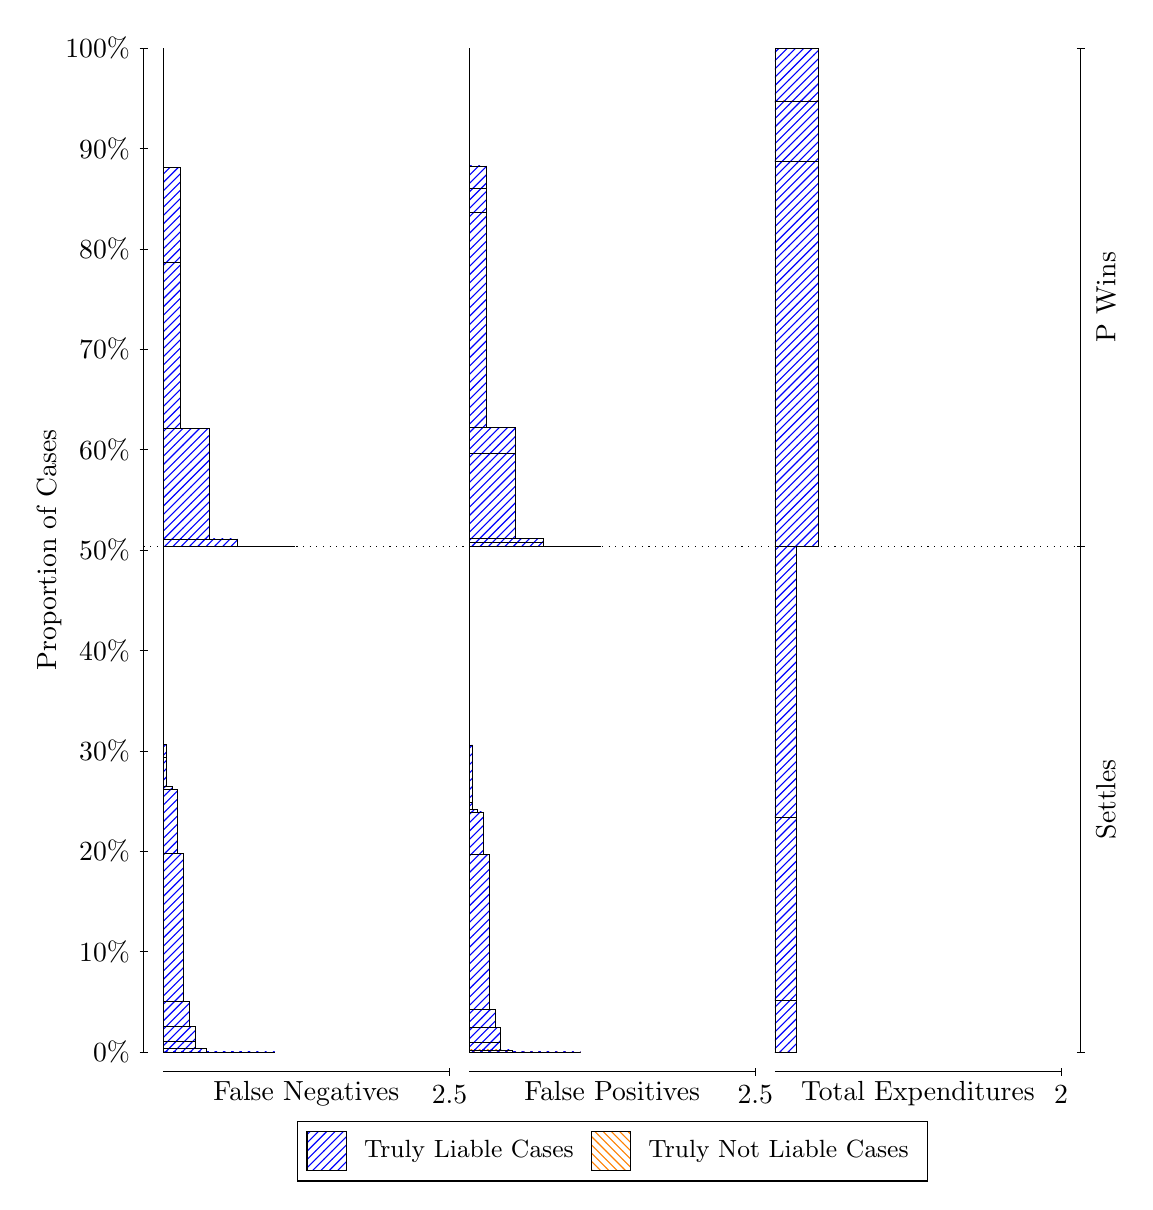
\begin{tikzpicture}
\draw[black, very thin] (1.5,1.75) -- (1.5,14.5);
\node[rotate=90, text=black, anchor=center] at (0.3, 8.125) {Proportion of Cases};
\draw[black, very thin] (1.45,1.75) -- (1.55,1.75);
\node[text=black, anchor=east] at (1.45, 1.75) {0\%};
\draw[black, very thin] (1.45,3.025) -- (1.55,3.025);
\node[text=black, anchor=east] at (1.45, 3.025) {10\%};
\draw[black, very thin] (1.45,4.3) -- (1.55,4.3);
\node[text=black, anchor=east] at (1.45, 4.3) {20\%};
\draw[black, very thin] (1.45,5.575) -- (1.55,5.575);
\node[text=black, anchor=east] at (1.45, 5.575) {30\%};
\draw[black, very thin] (1.45,6.85) -- (1.55,6.85);
\node[text=black, anchor=east] at (1.45, 6.85) {40\%};
\draw[black, very thin] (1.45,8.125) -- (1.55,8.125);
\node[text=black, anchor=east] at (1.45, 8.125) {50\%};
\draw[black, very thin] (1.45,9.4) -- (1.55,9.4);
\node[text=black, anchor=east] at (1.45, 9.4) {60\%};
\draw[black, very thin] (1.45,10.675) -- (1.55,10.675);
\node[text=black, anchor=east] at (1.45, 10.675) {70\%};
\draw[black, very thin] (1.45,11.95) -- (1.55,11.95);
\node[text=black, anchor=east] at (1.45, 11.95) {80\%};
\draw[black, very thin] (1.45,13.225) -- (1.55,13.225);
\node[text=black, anchor=east] at (1.45, 13.225) {90\%};
\draw[black, very thin] (1.45,14.5) -- (1.55,14.5);
\node[text=black, anchor=east] at (1.45, 14.5) {100\%};

\draw[black, very thin] (13.4,1.75) -- (13.4,14.5);
\draw[black, very thin] (13.35,1.75) -- (13.45,1.75);
\node[anchor=west] at (13.35, 1.75) {};
\draw[black, very thin] (13.35,8.1696) -- (13.45,8.1696);
\node[anchor=west] at (13.35, 8.1696) {};
\draw[black, very thin] (13.35,14.5) -- (13.45,14.5);
\node[anchor=west] at (13.35, 14.5) {};

\draw[black, very thin, pattern color=blue, pattern=north east lines] (1.75,1.75) rectangle (3.167,1.75);
\draw[black, very thin, pattern color=blue, pattern=north east lines] (1.75,1.75) rectangle (3.0217,1.75);
\draw[black, very thin, pattern color=blue, pattern=north east lines] (1.75,1.75) rectangle (2.8763,1.75);
\draw[black, very thin, pattern color=blue, pattern=north east lines] (1.75,1.75) rectangle (2.8037,1.75);
\draw[black, very thin, pattern color=blue, pattern=north east lines] (1.75,1.75) rectangle (2.731,1.75);
\draw[black, very thin, pattern color=blue, pattern=north east lines] (1.75,1.75) rectangle (2.6583,1.75);
\draw[black, very thin, pattern color=blue, pattern=north east lines] (1.75,1.75) rectangle (2.5857,1.75);
\draw[black, very thin, pattern color=blue, pattern=north east lines] (1.75,1.75) rectangle (2.513,1.7501);
\draw[black, very thin, pattern color=blue, pattern=north east lines] (1.75,1.7501) rectangle (2.4403,1.7524);
\draw[black, very thin, pattern color=blue, pattern=north east lines] (1.75,1.7524) rectangle (2.3677,1.7524);
\draw[black, very thin, pattern color=blue, pattern=north east lines] (1.75,1.7524) rectangle (2.295,1.7981);
\draw[black, very thin, pattern color=blue, pattern=north east lines] (1.75,1.7981) rectangle (2.2223,1.7993);
\draw[black, very thin, pattern color=blue, pattern=north east lines] (1.75,1.7993) rectangle (2.1497,1.8837);
\draw[black, very thin, pattern color=blue, pattern=north east lines] (1.75,1.8837) rectangle (2.1497,2.0788);
\draw[black, very thin, pattern color=blue, pattern=north east lines] (1.75,2.0788) rectangle (2.077,2.3957);
\draw[black, very thin, pattern color=blue, pattern=north east lines] (1.75,2.3957) rectangle (2.0043,2.396);
\draw[black, very thin, pattern color=blue, pattern=north east lines] (1.75,2.396) rectangle (2.0043,4.27);
\draw[black, very thin, pattern color=blue, pattern=north east lines] (1.75,4.27) rectangle (1.9317,5.0883);
\draw[black, very thin, pattern color=blue, pattern=north east lines] (1.75,5.0883) rectangle (1.859,5.1199);
\draw[black, very thin, pattern color=blue, pattern=north east lines] (1.75,5.1199) rectangle (1.7863,5.4866);
\draw[black, very thin, pattern color=blue, pattern=north east lines] (1.75,5.4866) rectangle (1.7863,5.6556);
\draw[black, very thin, pattern color=orange, pattern=north west lines] (1.75,5.6556) rectangle (1.75,5.6556);
\draw[black, very thin, pattern color=blue, pattern=north east lines] (1.75,5.6556) rectangle (1.75,8.1696);
\draw[black, very thin, pattern color=blue, pattern=north east lines] (1.75,8.1696) rectangle (3.4213,8.1696);
\draw[black, very thin, pattern color=blue, pattern=north east lines] (1.75,8.1696) rectangle (3.058,8.1705);
\draw[black, very thin, pattern color=blue, pattern=north east lines] (1.75,8.1705) rectangle (2.6947,8.2659);
\draw[black, very thin, pattern color=blue, pattern=north east lines] (1.75,8.2659) rectangle (2.3313,9.6663);
\draw[black, very thin, pattern color=blue, pattern=north east lines] (1.75,9.6663) rectangle (1.968,11.782);
\draw[black, very thin, pattern color=blue, pattern=north east lines] (1.75,11.782) rectangle (1.968,12.987);
\draw[black, very thin, pattern color=orange, pattern=north west lines] (1.75,12.987) rectangle (1.75,12.987);
\draw[black, very thin, pattern color=blue, pattern=north east lines] (1.75,12.987) rectangle (1.75,14.5);
\draw[black, very thin, pattern color=orange, pattern=north west lines] (5.6333,1.75) rectangle (7.0503,1.75);
\draw[black, very thin, pattern color=blue, pattern=north east lines] (5.6333,1.75) rectangle (7.0503,1.75);
\draw[black, very thin, pattern color=orange, pattern=north west lines] (5.6333,1.75) rectangle (6.905,1.75);
\draw[black, very thin, pattern color=blue, pattern=north east lines] (5.6333,1.75) rectangle (6.905,1.75);
\draw[black, very thin, pattern color=orange, pattern=north west lines] (5.6333,1.75) rectangle (6.7597,1.75);
\draw[black, very thin, pattern color=blue, pattern=north east lines] (5.6333,1.75) rectangle (6.7597,1.75);
\draw[black, very thin, pattern color=blue, pattern=north east lines] (5.6333,1.75) rectangle (6.687,1.75);
\draw[black, very thin, pattern color=orange, pattern=north west lines] (5.6333,1.75) rectangle (6.6143,1.75);
\draw[black, very thin, pattern color=blue, pattern=north east lines] (5.6333,1.75) rectangle (6.6143,1.75);
\draw[black, very thin, pattern color=blue, pattern=north east lines] (5.6333,1.75) rectangle (6.5417,1.75);
\draw[black, very thin, pattern color=orange, pattern=north west lines] (5.6333,1.75) rectangle (6.469,1.75);
\draw[black, very thin, pattern color=blue, pattern=north east lines] (5.6333,1.75) rectangle (6.469,1.75);
\draw[black, very thin, pattern color=blue, pattern=north east lines] (5.6333,1.75) rectangle (6.3963,1.7509);
\draw[black, very thin, pattern color=orange, pattern=north west lines] (5.6333,1.7509) rectangle (6.3237,1.7509);
\draw[black, very thin, pattern color=blue, pattern=north east lines] (5.6333,1.7509) rectangle (6.3237,1.7524);
\draw[black, very thin, pattern color=blue, pattern=north east lines] (5.6333,1.7524) rectangle (6.251,1.7524);
\draw[black, very thin, pattern color=orange, pattern=north west lines] (5.6333,1.7524) rectangle (6.1783,1.7524);
\draw[black, very thin, pattern color=blue, pattern=north east lines] (5.6333,1.7524) rectangle (6.1783,1.7765);
\draw[black, very thin, pattern color=blue, pattern=north east lines] (5.6333,1.7765) rectangle (6.1057,1.7777);
\draw[black, very thin, pattern color=orange, pattern=north west lines] (5.6333,1.7777) rectangle (6.033,1.7777);
\draw[black, very thin, pattern color=blue, pattern=north east lines] (5.6333,1.7777) rectangle (6.033,1.8752);
\draw[black, very thin, pattern color=blue, pattern=north east lines] (5.6333,1.8752) rectangle (6.033,2.0596);
\draw[black, very thin, pattern color=blue, pattern=north east lines] (5.6333,2.0596) rectangle (5.9603,2.2922);
\draw[black, very thin, pattern color=orange, pattern=north west lines] (5.6333,2.2922) rectangle (5.8877,2.2922);
\draw[black, very thin, pattern color=blue, pattern=north east lines] (5.6333,2.2922) rectangle (5.8877,4.2638);
\draw[black, very thin, pattern color=blue, pattern=north east lines] (5.6333,4.2638) rectangle (5.8877,4.264);
\draw[black, very thin, pattern color=blue, pattern=north east lines] (5.6333,4.264) rectangle (5.815,4.7997);
\draw[black, very thin, pattern color=blue, pattern=north east lines] (5.6333,4.7997) rectangle (5.7423,4.8313);
\draw[black, very thin, pattern color=blue, pattern=north east lines] (5.6333,4.8313) rectangle (5.6697,4.9158);
\draw[black, very thin, pattern color=blue, pattern=north east lines] (5.6333,4.9158) rectangle (5.6697,5.6496);
\draw[black, very thin, pattern color=blue, pattern=north east lines] (5.6333,5.6496) rectangle (5.6333,8.1696);
\draw[black, very thin, pattern color=orange, pattern=north west lines] (5.6333,8.1696) rectangle (7.3047,8.1696);
\draw[black, very thin, pattern color=blue, pattern=north east lines] (5.6333,8.1696) rectangle (7.3047,8.1696);
\draw[black, very thin, pattern color=orange, pattern=north west lines] (5.6333,8.1696) rectangle (6.9413,8.1696);
\draw[black, very thin, pattern color=blue, pattern=north east lines] (5.6333,8.1696) rectangle (6.9413,8.1699);
\draw[black, very thin, pattern color=blue, pattern=north east lines] (5.6333,8.1699) rectangle (6.9413,8.1706);
\draw[black, very thin, pattern color=orange, pattern=north west lines] (5.6333,8.1706) rectangle (6.578,8.1706);
\draw[black, very thin, pattern color=blue, pattern=north east lines] (5.6333,8.1706) rectangle (6.578,8.225);
\draw[black, very thin, pattern color=blue, pattern=north east lines] (5.6333,8.225) rectangle (6.578,8.2751);
\draw[black, very thin, pattern color=orange, pattern=north west lines] (5.6333,8.2751) rectangle (6.2147,8.2751);
\draw[black, very thin, pattern color=blue, pattern=north east lines] (5.6333,8.2751) rectangle (6.2147,9.3502);
\draw[black, very thin, pattern color=blue, pattern=north east lines] (5.6333,9.3502) rectangle (6.2147,9.6824);
\draw[black, very thin, pattern color=blue, pattern=north east lines] (5.6333,9.6824) rectangle (5.8513,12.411);
\draw[black, very thin, pattern color=orange, pattern=north west lines] (5.6333,12.411) rectangle (5.8513,12.411);
\draw[black, very thin, pattern color=blue, pattern=north east lines] (5.6333,12.411) rectangle (5.8513,12.715);
\draw[black, very thin, pattern color=blue, pattern=north east lines] (5.6333,12.715) rectangle (5.8513,13.003);
\draw[black, very thin, pattern color=blue, pattern=north east lines] (5.6333,13.003) rectangle (5.6333,14.5);
\draw[black, very thin, pattern color=orange, pattern=north west lines] (9.5167,1.75) rectangle (9.7892,1.75);
\draw[black, very thin, pattern color=blue, pattern=north east lines] (9.5167,1.75) rectangle (9.7892,2.407);
\draw[black, very thin, pattern color=orange, pattern=north west lines] (9.5167,2.407) rectangle (9.7892,2.407);
\draw[black, very thin, pattern color=blue, pattern=north east lines] (9.5167,2.407) rectangle (9.7892,4.7316);
\draw[black, very thin, pattern color=orange, pattern=north west lines] (9.5167,4.7316) rectangle (9.7892,4.7316);
\draw[black, very thin, pattern color=blue, pattern=north east lines] (9.5167,4.7316) rectangle (9.7892,8.1696);
\draw[black, very thin, pattern color=orange, pattern=north west lines] (9.5167,8.1696) rectangle (10.062,8.1696);
\draw[black, very thin, pattern color=blue, pattern=north east lines] (9.5167,8.1696) rectangle (10.062,13.056);
\draw[black, very thin, pattern color=orange, pattern=north west lines] (9.5167,13.056) rectangle (10.062,13.056);
\draw[black, very thin, pattern color=blue, pattern=north east lines] (9.5167,13.056) rectangle (10.062,13.828);
\draw[black, very thin, pattern color=orange, pattern=north west lines] (9.5167,13.828) rectangle (10.062,13.828);
\draw[black, very thin, pattern color=blue, pattern=north east lines] (9.5167,13.828) rectangle (10.062,14.5);
\draw[black, dotted] (1.5,8.1696) -- (13.4,8.1696);
\draw[black, very thin] (1.75,1.5) -- (5.3833,1.5);
\node[text=black, anchor=north] at (3.5667, 1.5) {False Negatives};
\draw[black, very thin] (5.3833,1.45) -- (5.3833,1.55);
\node[text=black, anchor=north] at (5.3833, 1.45) {2.5};

\draw[black, very thin] (5.6333,1.5) -- (9.2667,1.5);
\node[text=black, anchor=north] at (7.45, 1.5) {False Positives};
\draw[black, very thin] (9.2667,1.45) -- (9.2667,1.55);
\node[text=black, anchor=north] at (9.2667, 1.45) {2.5};

\draw[black, very thin] (9.5167,1.5) -- (13.15,1.5);
\node[text=black, anchor=north] at (11.333, 1.5) {Total Expenditures};
\draw[black, very thin] (13.15,1.45) -- (13.15,1.55);
\node[text=black, anchor=north] at (13.15, 1.45) {2};

\node[text=black, centered, rotate=90] at (13.72, 4.9598) {Settles};
\node[text=black, centered, rotate=90] at (13.72, 11.335) {P Wins};

\draw (7.449999999999999,1.5) node[draw=none] (baseCoordinate) {};
\begin{scope}[align=center]
        \matrix[scale=0.5, draw=black, below=0.5cm of baseCoordinate, nodes={draw}, column sep=0.1cm]{
            \node[rectangle, draw, minimum width=0.5cm, minimum height=0.5cm, pattern color=blue, pattern=north east lines] {}; &
            \node[draw=none, font=\small, text=black] (B) {Truly Liable Cases}; &
            \node[rectangle, draw, minimum width=0.5cm, minimum height=0.5cm, pattern color=orange, pattern=north west lines] {}; &
            \node[draw=none, font=\small, text=black] (B) {Truly Not Liable Cases}; \\
            };
\end{scope}

\end{tikzpicture}
\end{document}